\documentclass[journal=jpcafh,manuscript=article]{achemso}
\usepackage[english]{babel}
\usepackage{amsmath}
\usepackage{amsfonts}
\usepackage{amssymb}
\usepackage[T1]{fontenc}
\usepackage[utf8]{inputenc}
\usepackage{lmodern}
\usepackage{graphicx}
\usepackage{epstopdf}
\usepackage{natbib}

\graphicspath{ {./images/} }

\SectionNumbersOn

\author{Franz Martinez}
\email{franzmichel.martinez@ucalgary.ca}
\affiliation{Schulich School of Engineering, University of Calgary, Calgary, Alberta, Canada}
\title{Outline--Draft JCP format for: Reactive Force Field for Solid Oxides Containing Lanthanum}

\begin{document}

\begin{abstract}
\textbf{abstract needs to be updated}


In this work, we perform the parametrization of a reactive force field, ReaxFF, for Lanthanum and its oxides.
We describe the procedure followed and provide results that validate the derived parameters in their ability to describe bulk structures, surfaces, and nanoparticles.
Comparison of our results using ReaxFF and electronic structure methods show good agreement in the reproduction of surfaces energies and bulk modulus; with the latter showing good agreement with experimentally reported results.
We also show that our parametrization is able to capture the trend in adsorption energies between Lanthanum oxides and adsorbates like methane and water \textbf{to be obtained}.
These results highlight the utility of ReaxFF to study systems containing Lanthanum and provide a significant addition to reactive molecular dynamics for studying properties and even redox properties on Lanthanum oxide surfaces.

\end{abstract}


\section{Introduction}

% introduce lanthanum uses
Lanthanum is a transition metal involved in various applications that range from use in catalysts, batteries, and in medicine \cite{atwood2013rare,he2013preparation}.
Particularly, catalysts based on Lanthanum oxide have shown a good efficiency in the oxidative coupling of methane to form ethane and/or ethylene \textbf{import citation}, or as main components of electro--catalysts used in CO$_2$ conversion to CO \textbf{import citation}.

% what is the problem with lanthanum
\emph{need to introduce more about uses of La}

Quantum mechanical calculations have been carried out to understand the role and influence, if any, of Lanthanum on its many applications.
However, many of the phenomena that takes place in catalysis involve the interaction of many atoms for which rigorous quantum mechanical calculations are unfeasible.
For this reason, force fields are commonly used to study applications via molecular dynamics calculations.
In particular, the behaviour of La$^3+$ in aqueous solution has been studied by various groups using different parametrization strategies to improve the accuracy of the description of the interaction between Lanthanum and water \cite{duvail2007pair}.
These approaches have proven to successfully describe the La--O interaction in liquid water, but due to the size of Lanthanum the introduction of some form of explicit polarizability is necessary to properly describe the interactions between Lanthanum and other elements.

One of the major drawbacks of the use of general polarizable force fields is the impossibility to describe chemical reactions, as these models disable explicit bond breaking and formation to produce transferable parameters and simple expressions for calculating energies and forces.
But, with the increasing computational power processing, reactive force fields that can capture bond breaking and formation on--the--fly have been developed actively during the last decade.
Particularly, ReaxFF is a reactive force field that has been extensively used to study successfully reactive events between solid, liquid, and gas phases.
This transferability between phases, and the possibility to study phenomena where chemical events and dynamical factors are of importance makes ReaxFF a powerful tool that bridges the lower computational expense from force fields and the quantum mechanical description of a system.
Although the current form of ReaxFF has been in development since 2008 \cite{chenoweth_reaxff_2008} and many elements have been parametrized to be used in ReaxFF not all interactions have been fully parametrized, and some elements still remain to be parametrized.
An important point is that parameters used in ReaxFF are heavily dependent on the applications for which they have been explicitly parametrized, so while some parameters can be transferable testing is necessary to ensure that interactions are well described.

The purpose of this study is to generate a set of parameters for Lanthanum as well as its interaction with other elements, namely Ca, Fe, Cr, and O, to be used for describing solid state materials used in catalysis.
To this end, in the remainder of this paper, we introduce ReaxFF and a parametrization strategy in Sec.~\ref{sec:reaxff-strategy}; and the computational methods used, i.e. electronic structure calculations in Sec.~\ref{sec:dft-details}; and molecular dynamics simulations in Sec.~\ref{sec:md-details}.
Then, we discuss in Sec.~\ref{sec:results-and-discussion} the quality of the newly generated parameters by analyzing the ability of the ReaxFF to reproduce the generated dataset from quantum mechanical calculations.
Finally, we use the parameters obtained to model some possible applications discuss the results in Sec.~\ref{sec:applications}, and present our concluding remarks in Sec.~\ref{sec:conclusions}

%CO$_2$, electrocatalysts, and solid oxide fuels.\cite{
%habisreutinger_photocatalytic_2013,
%e.benson_electrocatalytic_2009,
%pradeepindrakanti_photoinduced_2009,
%indrakanti_quantum_2009,
%zeng_review_2018,
%yamada_systematic_2018,
%kar_enhanced_2016,
%grimaud_double_2013,
%ni_electrochemical_2012,
%tan_co_2011,
%baniecki_photoemission_2008,
%jia_heterogeneous_2017,
%yin_oxide_2018,
%zheng_review_2017,
%andersson_review_2010,
%beatriz_microwave-assisted_2015}
%
%DFT studies.\cite{tian_dft_2018,
%mayeshiba_strain_2017,
%wang_oxidation_2006,
%li_density_2013,
%liu_influence_2018,
%seo_design_2015,
%evarestov_adsorption_2007,
%pilania_establishing_2012,
%pilania_adsorption_2010,
%zurek_predicting_2015}
%
%Molecular dynamics studies.\cite{wang_coarse-grained_2014}

\section{Computational Methods}

\subsection{ReaxFF and Parameterization Strategy}
\label{sec:reaxff-strategy}

ReaxFF is a force field based on the dynamical computation of the bond-order, which dictates the connectivity between atoms on the fly.
This approach allows ReaxFF to consider bond breaking and formation, and therefore the ability to follow the apparition of intermediates involved in the reaction mechanism in complex systems containing thousands of atoms.\cite{migliorati_development_2017,merinov_reaxff_2014,
raymand_reactive_2008,
shin_development_2015,
van_duin_reaxff_2008,
goddard_development_2006,
hubin_parameterization_2016,
senftle_reaxff_2016,
chenoweth_reaxff_2009,
chenoweth_reaxff_2008,
van_duin_reaxff_2008-1,
liu_reaxff-lg:_2011}

Its use bridges the advantages of classical molecular dynamics simulation with those of quantum--mechanical approaches.

Parametrization of ReaxFF involves generation of a dataset, generally from quantum mechanical calculations, and subsequent fitting of the force field parameters with respect to the dataset by minimizing the error function, $E_f$,
\begin{equation}
E_f = \frac{(x_{i} - x_{ReaxFF,i})^2}{w_i}.
\end{equation}
Where $x_{i}$ is the value of a property $x$ (e.g. heat of formation, geometries, energetic differences, etc.); $x_{ReaxFF,i}$ is such property calculated using ReaxFF; and $w_i$ is the weight, or accuracy, associated to the desired deviation between both $x_i$ and $x_{ReaxFF,i}$
In this work the Monte Carlo Force Field Optimizer,\cite{iype_parameterization_2013} part of the ADF package, has been used to fit the various parameters of the force field, mostly because the method has been shown to give good results independent of the initial guess for the force fields parameters.

The parametrization of the force field was performed using various stages, and it started with known parameters for C, H, O, S, Fe, and Cr from a previous study of hydrocarbon oxidation on pyrite--covered Cr$_2$O$_3$; \cite{shin_development_2015} and for Ca from a previous study of calcium oxyde hydration. \cite{manzano_hydration_2012}

With starting parameters for most elements except for La, the first stage of the parametrization involved fitting the La--La parameters of the force field to the following: quantum mechanically calculated equations of state corresponding to three solid phases of La, i.e. double hexagonal close packed (dhcp, $\alpha$-La), face centered cubic (fcc, $\gamma$-La), and body centered cubic (bcc, $\beta$-La); and data from the electronic structure calculation of the La$_2$ molecule was added.
This stage was carried out while keeping parameters for other interactions unchanged.
The following stage involved further fitting of the La--La parameters, namely those related to the electrostatic interaction (EEM shielding, EEM electronegativity, and EMM hardness), and the La--O parameters by adding to the dataset Mulliken charges and geometrical information obtained from the optimized structures of the La$_2$O$_3$ cluster, three La$_4$O$_6$ clusters, and one La$_6$O$_9$ cluster.
Also, the equations of state corresponding to two solid structures of La$_2$O$_3$ were computed and added.


\subsection{Electronic Structure Calculations for Dataset Generation}
\label{sec:dft-details}

DFT calculations are carried out using Quantum Espresso,\cite{giannozzi_advanced_2017} for all solid structures in bulk or slab form.
These calculations were performed using the pseudo--potentials from the PSlibrary including scalar-relativistic effects due to the presence of Lanthanum \textbf{put references}.
A value of 75.0 Ry was used for the kinetic energy cutoff, which was tested for convergence ensuring that $\Delta E_{tot} / \Delta E_{cut} <$ 0.01 eV was obtained per atom.
Monkhorst-Pack k-point sampling of the Brillouin zone was chosen to be $4\times4\times4$ for most calculations.
The criterion used involved using a k-point grid of 4 on the edge of a cell between 5 and 8 \AA in length, then to preserve the grid on bigger or smaller cells, the grid was scaled accordingly.
The k-point grids used were also tested using the same criterion from energy converge to ensure convergence with respect to grid size.

Because the transition metals present localized electronic density on their d--orbitals with strong correlation, the Hubbard correction is employed to take into account these effects.\textbf{put references}
Values used for the Hubbard term, U, were taken from \textbf{put values, and justify about not determining their values from linear response theory}

The convergence criterion used for all calculations was of 0.02 eV for the total energy, and in the case of relaxations the maximum force component on each atom had to satisfy being smaller than 0.01 eV/\AA 

Differences in energies and optimized geometries were also obtained from clusters in the gas phase using \emph{Gaussian16} \textbf{put references}.
For these calculations, the B3LYP functional has been used with the aug--cc--pVTZ basis functions for oxygen and for lanthanum the La basis set from the Stuttgart/Dresden group, La(RSC97) \textbf{double check} with a 28--electron ECP \textbf{citation}.
By using this approach, we ensure that the parameters obtained for lanthanum in these calculations are consistent with the way the oxygen parameters were obtained in previous studies.

\subsection{Molecular Dynamics Trajectories Using ReaxFF}
\label{sec:md-details}

For the molecular dynamics simulations using ReaxFF, the system \textbf{specify details for bulk simulations and slabs} ... first is equilibrated using classical molecular dynamics with the UFF force field.
From the equilibrated trajectory at the conditions required \textbf{double check temperature and pressure and change this part}, several points are selected randomly as starting points for the simulation.
This ensures that the system starts from a correct point in equilibrium of the ensemble for the ReaxFF dynamics.

\section{Parametrization Results and Discussion}
\label{sec:results-and-discussion}

\subsection{Equations of State}

Equations of state for hexagonal La, LaFeO$_3$, LaCrO$_3$, ... were calculated using DFT, and the ReaxFF force field was parametrized to reproduce this curve to the best possible fit.
Because the relationship between energy and volume in solids allow to capture the stability of the phase, fitting of these curves give ReaxFF the ability to model accurately the bulk phase of the perovskite.

\begin{figure}[hbtp]
\centering
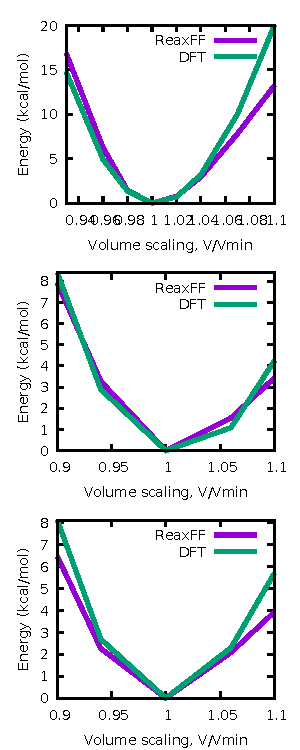
\includegraphics[scale=1]{three-La-eos.pdf}
\caption{Calculated equations of state corresponding to crystalline La in hexagonal (top), fcc (middle), and bcc (bottom) forms.}
\label{fig:laeos}
\end{figure}

The equations of state for the three forms of Lanthanum are presented in Fig.~\ref{fig:laeos}.
The plots show the parabolic behaviour of the equation of state, and that the parametrized ReaxFF can reproduce the results from DFT within an acceptable margin of error.
As for the trends in stability of the three phases, ReaxFF is unable to properly reproduce it.
The reported experimental trend places $\alpha$-La as the most stable, followed by $\gamma$-La, and then by$\beta$-La.
In the case of ReaxFF the trend goes from most stable to less stable as $\gamma$-La, $\beta$-La, and $\alpha$-La.
While the inability to reproduce stability is a known issue in ReaxFF, it is worth mentioning that in the case of La, the differences in energy between the phases is in the order of $\approx$~0.5~kcal/mol.
It is then unsurprising that the parametrized force field is unable to exactly reproduce the trend,  given how small the difference in energy is compared to the target error in the fitting of the force field, which averages around 5~kcal/mol.

The bulk modulus for $\alpha$-La was obtained by fitting the calculated points to the Birch-Murnaghan equation of state\cite{fu_first-principles_1983}, and the value obtained of 25.6\,GPa agrees with an approximate 8\% of error compared to the reported experimental bulk modulus value of 27.9\,GPa.\cite{lide2003crc}

\subsection{Surface Energies}

Given the differences, in structure and energetics, of the surface compared to the bulk, it is necessary to introduce this behaviour to the force field.
To this end, slabs of various perovskites were constructed from their bulk counterparts to extend the ReaxFF force field.
\textbf{Calculations currently going on}

\subsection{Oxygen Vacancy Formation Energies}

Introduction of Ca in the A--site of the perovskites favours the formation of oxygen vacancies due to the change in ionic size compared to La and the different charges of these cations. \textbf{cite}
Also, the formation of oxygen vacancies allow for ionic diffusion through the solid, which is an important process present when these solids are used as electrodes in solid oxide fuel or electrolysis cells.
The existence of oxygen vacancies in the system needs to be captured by ReaxFF in the form of correctly capturing changes in the chemical environment and in the relative stability of the solid unit cell in the absence of one oxygen.
For various perovskites, the oxygen vacancy formation energy is calculated and incorporated into the dataset used to fit ReaxFF.

\section{Applications}
\label{sec:applications}

\subsection{Nanoparticle formation of La$_2$O$_3$}



\subsection{Oxygen Diffusion through the Perovskites}

To exemplify the dynamics on the bulk, diffusion of O$_2^{-2}$ is followed through the perovskite in bulk phase.
Also, to account for the accuracy of the force field, the expansion coefficient is computed for LCFCr and this value is compared to experimental results.

\subsection{CO$_2$ Interactions on the Surface}

\textbf{this may be ommited for a future paper}

Using a slab of a representative portion \textbf{fill in details of the real size} of the surface of the LCFCr, various mixtures of gases are fed into one of the surfaces ...

Formation of intermediates is observed at 1073 K \textbf{double check temperature}

\section{Concluding Remarks}
\label{sec:conclusions}


\begin{acknowledgement}
This work has been enabled by the use of computing resources provided by Compute Canada.
\end{acknowledgement}

\pagebreak

\bibliography{co2perov2}

\pagebreak
\begin{tocentry}
\begin{center}
%\includegraphics{toc.eps}
insert ToC if requested
\end{center}
\end{tocentry}


\end{document}